\documentclass[ignorenonframetext,t]{beamer}
\setbeamertemplate{caption}[numbered]
\setbeamertemplate{caption label separator}{: }
\setbeamercolor{caption name}{fg=normal text.fg}
\beamertemplatenavigationsymbolsempty
\usepackage{lmodern}
\usepackage{amssymb,amsmath}
\usepackage{ifxetex,ifluatex}
\usepackage{fixltx2e} % provides \textsubscript
\ifnum 0\ifxetex 1\fi\ifluatex 1\fi=0 % if pdftex
  \usepackage[T1]{fontenc}
  \usepackage[utf8]{inputenc}
\else % if luatex or xelatex
  \ifxetex
    \usepackage{mathspec}
  \else
    \usepackage{fontspec}
  \fi
  \defaultfontfeatures{Ligatures=TeX,Scale=MatchLowercase}
\fi
\usetheme[]{Boadilla}
\usecolortheme{dove}
\usefonttheme{structuresmallcapsserif}
% use upquote if available, for straight quotes in verbatim environments
\IfFileExists{upquote.sty}{\usepackage{upquote}}{}
% use microtype if available
\IfFileExists{microtype.sty}{%
\usepackage{microtype}
\UseMicrotypeSet[protrusion]{basicmath} % disable protrusion for tt fonts
}{}
\newif\ifbibliography
\hypersetup{
            pdftitle={Theories as Ordinal Constraint},
            pdfauthor={Julia M. Haaf},
            pdfborder={0 0 0},
            breaklinks=true}
\urlstyle{same}  % don't use monospace font for urls
\usepackage{graphicx,grffile}
\makeatletter
\def\maxwidth{\ifdim\Gin@nat@width>\linewidth\linewidth\else\Gin@nat@width\fi}
\def\maxheight{\ifdim\Gin@nat@height>\textheight0.8\textheight\else\Gin@nat@height\fi}
\makeatother
% Scale images if necessary, so that they will not overflow the page
% margins by default, and it is still possible to overwrite the defaults
% using explicit options in \includegraphics[width, height, ...]{}
\setkeys{Gin}{width=\maxwidth,height=\maxheight,keepaspectratio}

% Prevent slide breaks in the middle of a paragraph:
\widowpenalties 1 10000
\raggedbottom

\AtBeginPart{
  \let\insertpartnumber\relax
  \let\partname\relax
  \frame{\partpage}
}
\AtBeginSection{
  \ifbibliography
  \else
    \let\insertsectionnumber\relax
    \let\sectionname\relax
    \frame{\sectionpage}
  \fi
}
\AtBeginSubsection{
  \let\insertsubsectionnumber\relax
  \let\subsectionname\relax
  \frame{\subsectionpage}
}

\setlength{\parindent}{0pt}
\setlength{\parskip}{6pt plus 2pt minus 1pt}
\setlength{\emergencystretch}{3em}  % prevent overfull lines
\providecommand{\tightlist}{%
  \setlength{\itemsep}{0pt}\setlength{\parskip}{0pt}}
\setcounter{secnumdepth}{0}
\usepackage{bm}
\usepackage{pcl}
\usepackage{amsmath}
\usepackage{setspace}
\usepackage{multirow}
\usepackage{xcolor}
\usepackage{adjustbox}
\titlegraphic{\centering \includegraphics[height=2cm, width=5.5cm]{pics/MULogoBig.png}}
\setbeamerfont{author}{series=\bfseries,parent=structure}
\setbeamerfont{frametitle}{size=\Large}
\setbeamerfont{title}{size = \Huge}

\title{Theories as Ordinal Constraint}
\subtitle{A Bayes Factor Approach}
\author{Julia M. Haaf}
\date{}

\begin{document}
\frame{\titlepage}

\begin{frame}{Testing Theories Using Ordinal Constraint}

\vspace*{1cm}

\begin{itemize}[<+->]
\tightlist
\item
  Is there a \emph{true} effect?
\item
  Example: Inhibition
  (\(\rightarrow \rightarrow \boldsymbol{\leftarrow} \rightarrow \rightarrow\)
  vs.
  \(\leftarrow \leftarrow \boldsymbol{\leftarrow} \leftarrow \leftarrow\))
\item
  What size is the \emph{true} effect?
\item
  4 ms vs.~40 ms. vs.~400 ms. ?
\item
  The size of the effect is rarely target of psychological theory
\item
  Is the \emph{true} effect in the expected direction?
\item
  \textbf{Idea: Stating theory as multiple, simultaneous ordinal
  constraint}
\end{itemize}

\vspace*{.5cm}

\centering \includegraphics[width = 50px]{pics/Direction.png}

\end{frame}

\begin{frame}{A psychologist's favorite design}

\framesubtitle{With Ugly Bugs}

\vspace*{.5cm}

\centering \includegraphics[width = 120px]{pics/newBug.png}

\end{frame}

\begin{frame}{A psychologist's favorite design}

\framesubtitle{Ryan, Wilde, \& Crist (2013)}

\vspace*{1cm}

\centering

\begin{tabular}{llcc}
\hline
& & \multicolumn{2}{c}{\bf{Disgust}} \\ \cline{2-4}
& & Low & High\\ \hline
\multirow{2}{*}{\bf{Fear}} & Low & Low/Low & Low/High \\
& High & High/Low & High/High    \\ \hline
\end{tabular}

\vspace*{1.8cm}

\centering \includegraphics[origin=c, angle = 90, width = 250px]{pics/newBug.png}

\end{frame}

\begin{frame}{A psychologist's favorite design}

\framesubtitle{Ryan, Wilde, \& Crist (2013)}

\vspace*{1cm}

\centering

\begin{tabular}{llcc}
\hline
& & \multicolumn{2}{c}{\bf{Disgust}} \\ \cline{2-4}
& & Low & High\\ \hline
\multirow{2}{*}{\bf{Fear}} & Low & Low/Low & Low/High \\
& High & High/Low & High/High    \\ \hline
\end{tabular}

\vspace*{.8cm}

\bf{"How willing are you to kill/get rid of this bug?"}

\vspace*{.4cm}

\centering \includegraphics[origin=c, angle = 90, width = 250px]{pics/newBug.png}

\end{frame}

\begin{frame}{Systems of Orders with Bugs}

\vspace*{.5cm}

\includegraphics{t_files/figure-beamer/fig-1-1.pdf}

\end{frame}

\begin{frame}{Systems of Orders with Bugs}

\vspace*{.5cm}

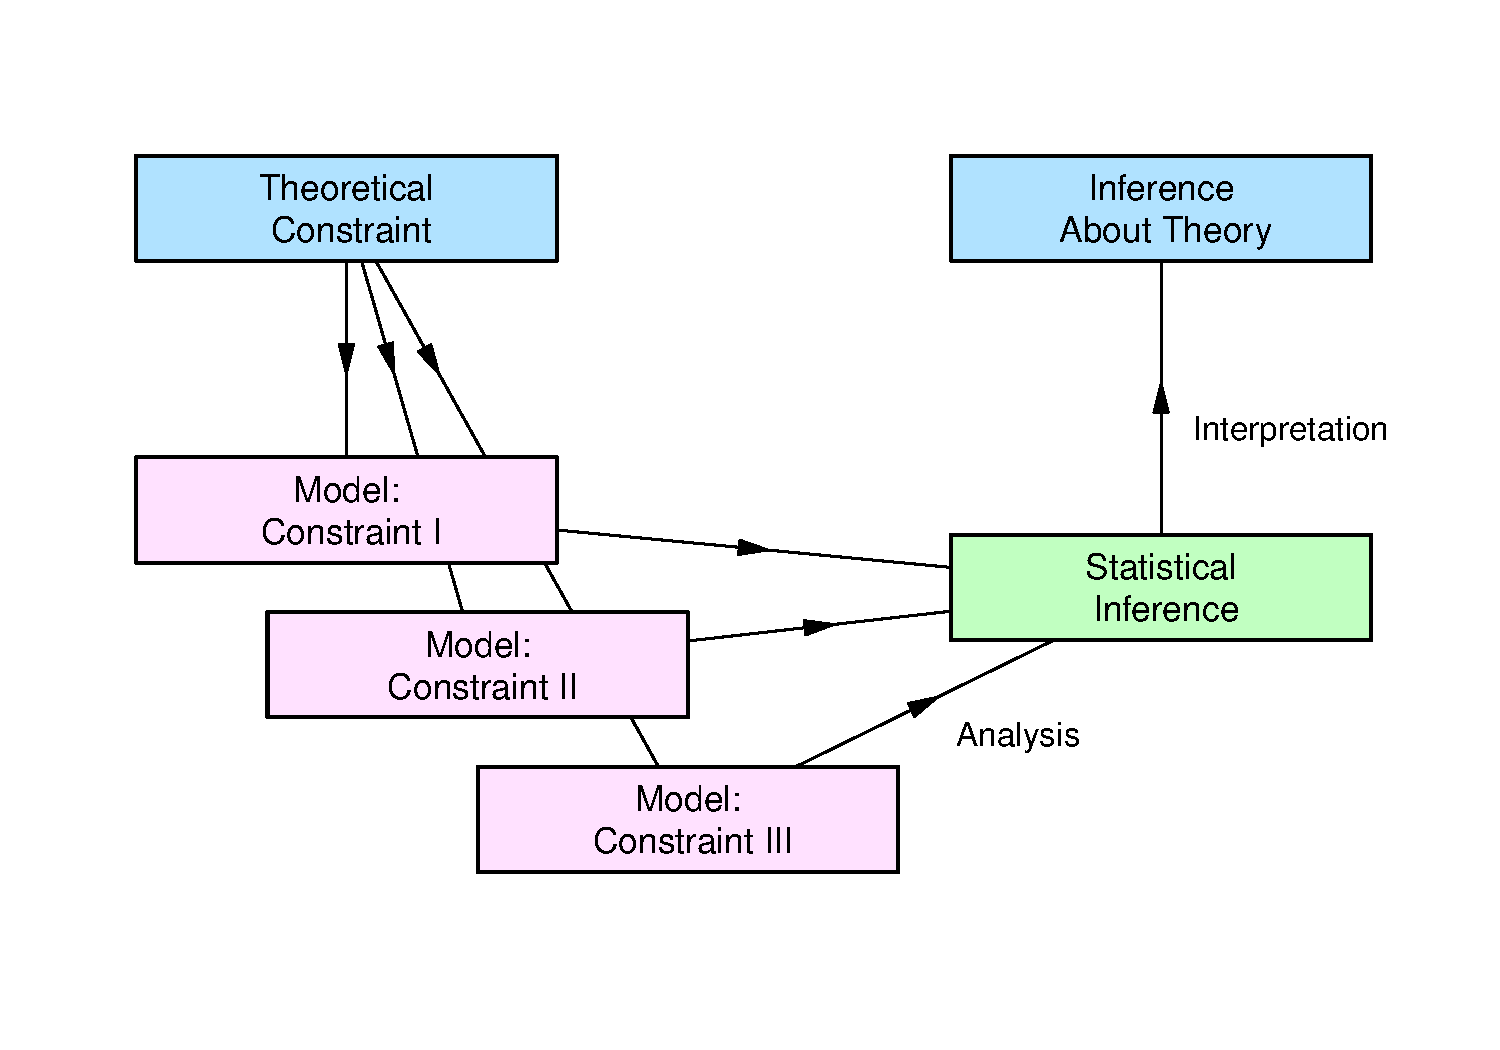
\includegraphics{t_files/figure-beamer/unnamed-chunk-2-1.pdf}

\end{frame}

\begin{frame}{Systems of Orders with Bugs}

\vspace*{.5cm}

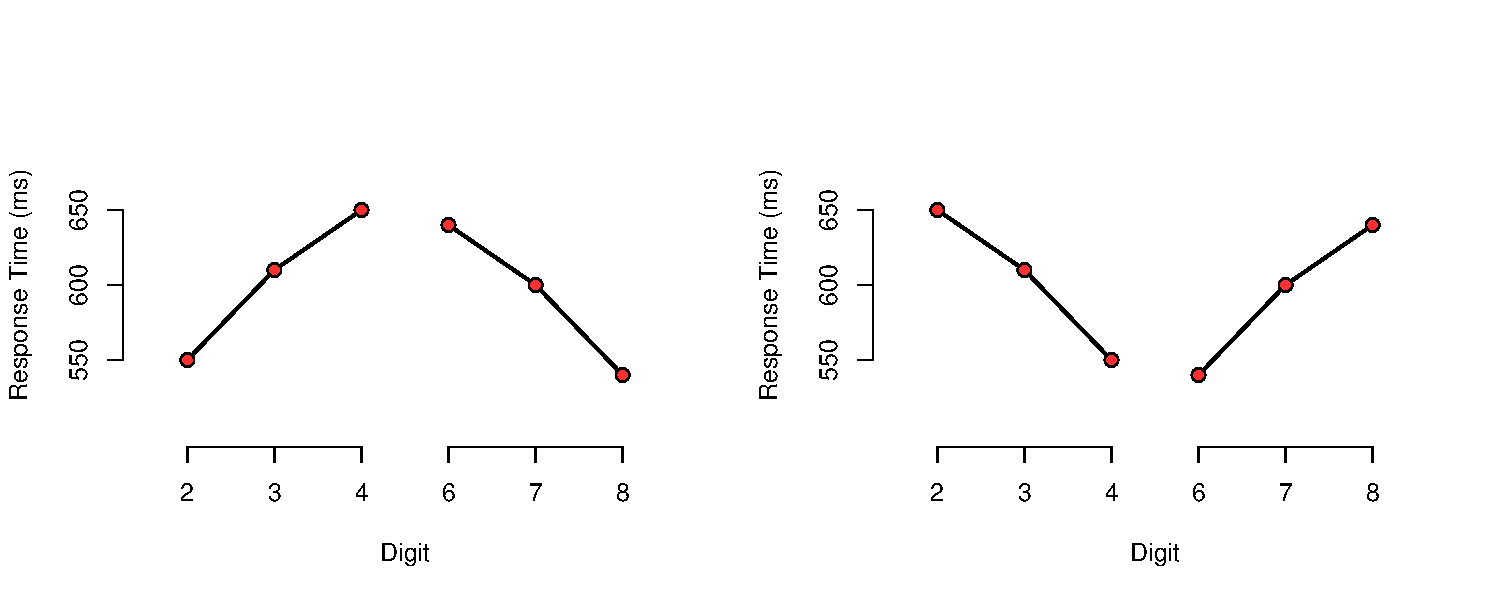
\includegraphics{t_files/figure-beamer/unnamed-chunk-3-1.pdf}

\end{frame}

\begin{frame}{Systems of Orders with Bugs}

\vspace*{.5cm}

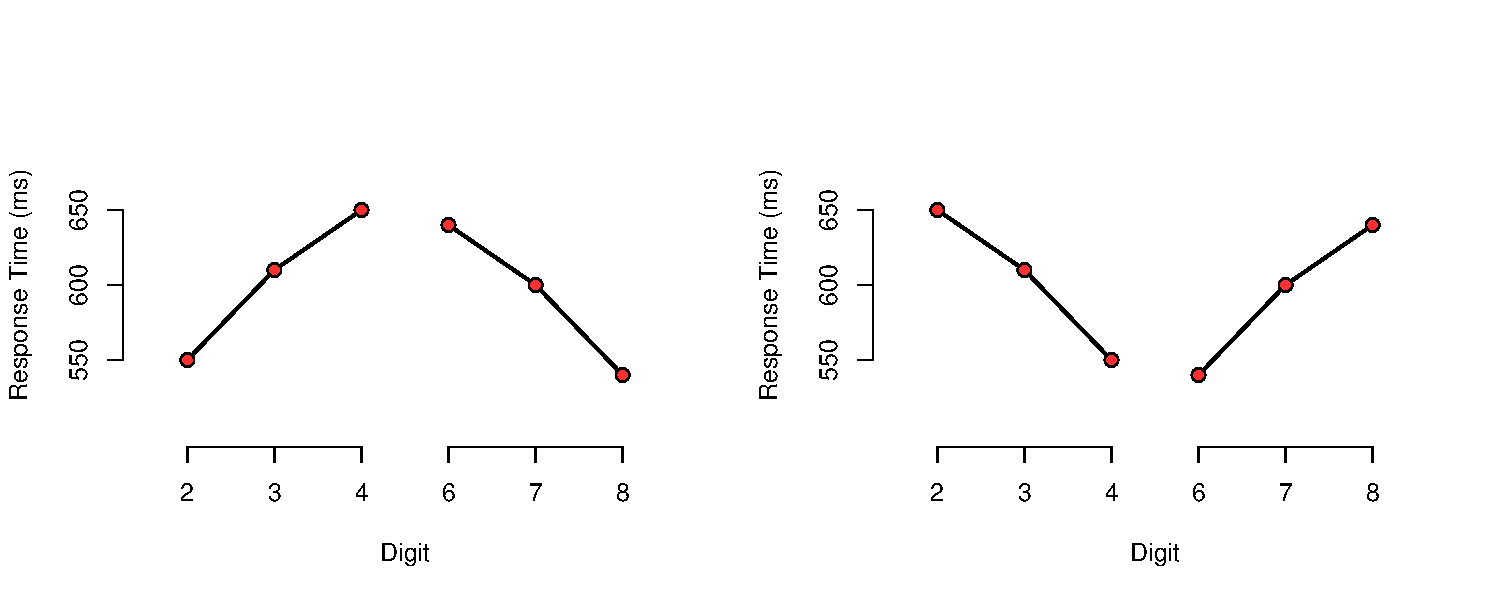
\includegraphics{t_files/figure-beamer/unnamed-chunk-4-1.pdf}

\end{frame}

\begin{frame}{Systems of Orders with Bugs}

\vspace*{.5cm}

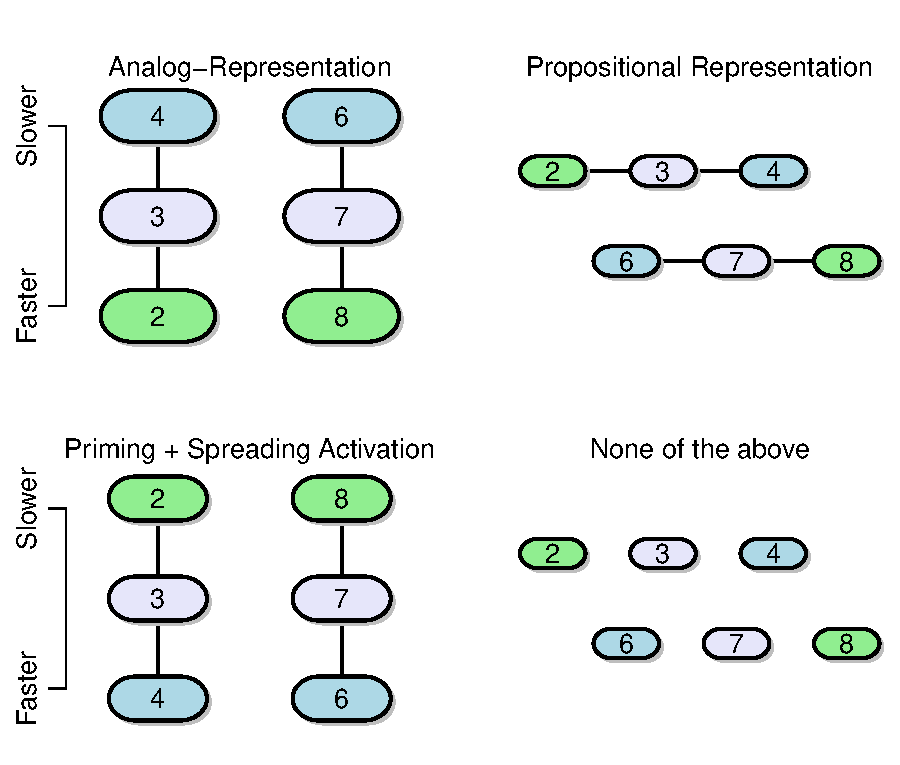
\includegraphics{t_files/figure-beamer/unnamed-chunk-5-1.pdf}

\end{frame}

\begin{frame}{Systems of Orders with Bugs}

\vspace*{.5cm}

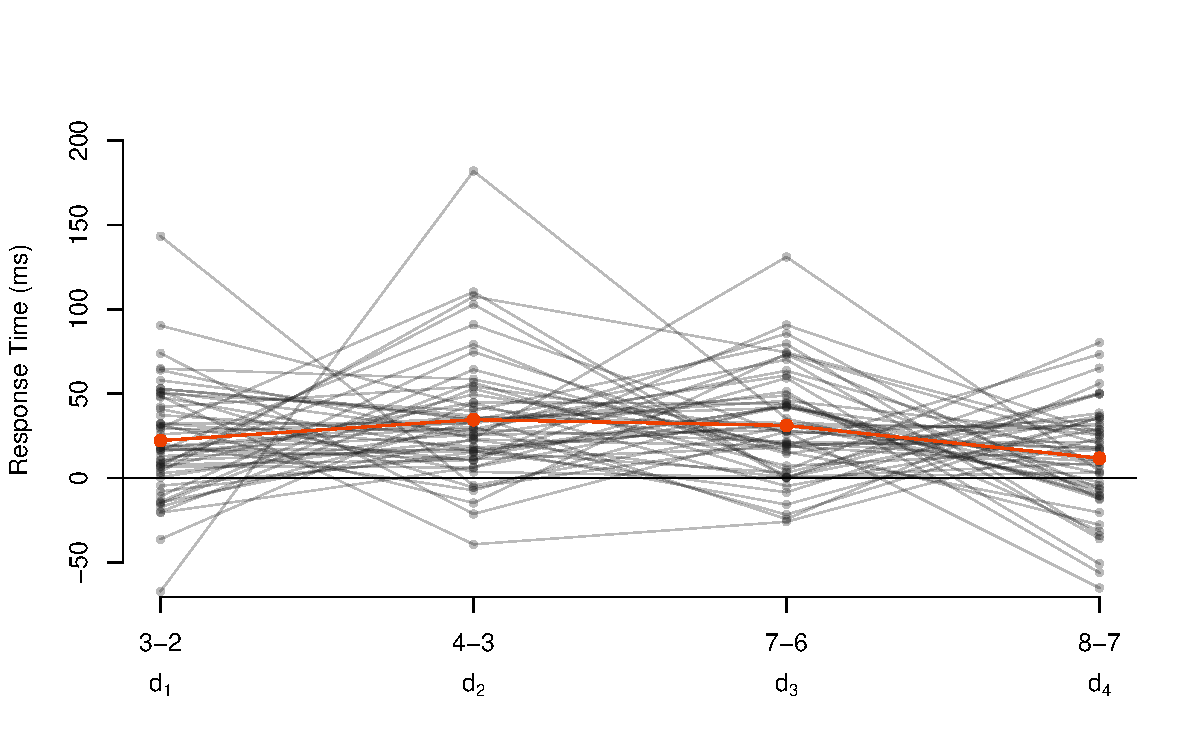
\includegraphics{t_files/figure-beamer/unnamed-chunk-6-1.pdf}

\end{frame}

\begin{frame}{Systems of Order Analysis with Bugs}

\framesubtitle{Data}

\vspace*{.5cm}

\begin{columns}
\column{.1\textwidth}
\column{.8\textwidth}













\begin{center}\includegraphics{t_files/figure-beamer/plot-bugs-1} \end{center}

\column{.1\textwidth}
\end{columns}

\end{frame}

\begin{frame}{Assessing systems of orders with Bayesian analysis}

\vspace*{1cm}

\begin{figure}
\centering
\begin{minipage}{.6\textwidth}

\begin{itemize}
\item Assessing ordinal constraints is straight-forward in Bayesian analysis
\item Take posterior samples from the unconstrained model
\item What proportion obeys the ordinal constraint in the posterior as compared to the prior?
\end{itemize}

\end{minipage}%
\begin{minipage}{.4\textwidth}
  \centering
  \includegraphics[width = 90px]{pics/book.jpg}
\end{minipage}
\end{figure}

\end{frame}

\begin{frame}{Systems of Order Analysis with Bugs}

\framesubtitle{Results}

\vspace*{.5cm}

\begin{itemize}[<+->]
\tightlist
\item
  Preferred model: \textbf{Consistent postitive} model (\(M_1\))
\end{itemize}

\begin{itemize}[<+->]
\tightlist
\item
  Preferred 2.98-to-1 over the \textbf{positive equality} model
  (\(M_2\))
\item
  Preferred 3.64-to-1 over the \textbf{fear only} model (\(M_3\))
\item
  Preferred 5.20-to-1 over the \textbf{unconstrained model} (\(M_5\))
\item
  Preferred 11261-to-1 over the \textbf{disgust only} model (\(M_4\))
\item
  Preferred 50808-to-1 over the \textbf{null} model (\(M_0\))
\end{itemize}

\end{frame}

\begin{frame}{Preferred model}

\vspace*{1cm}

\begin{columns}
\column{.3\textwidth}
\column{.4\textwidth}


\begin{center}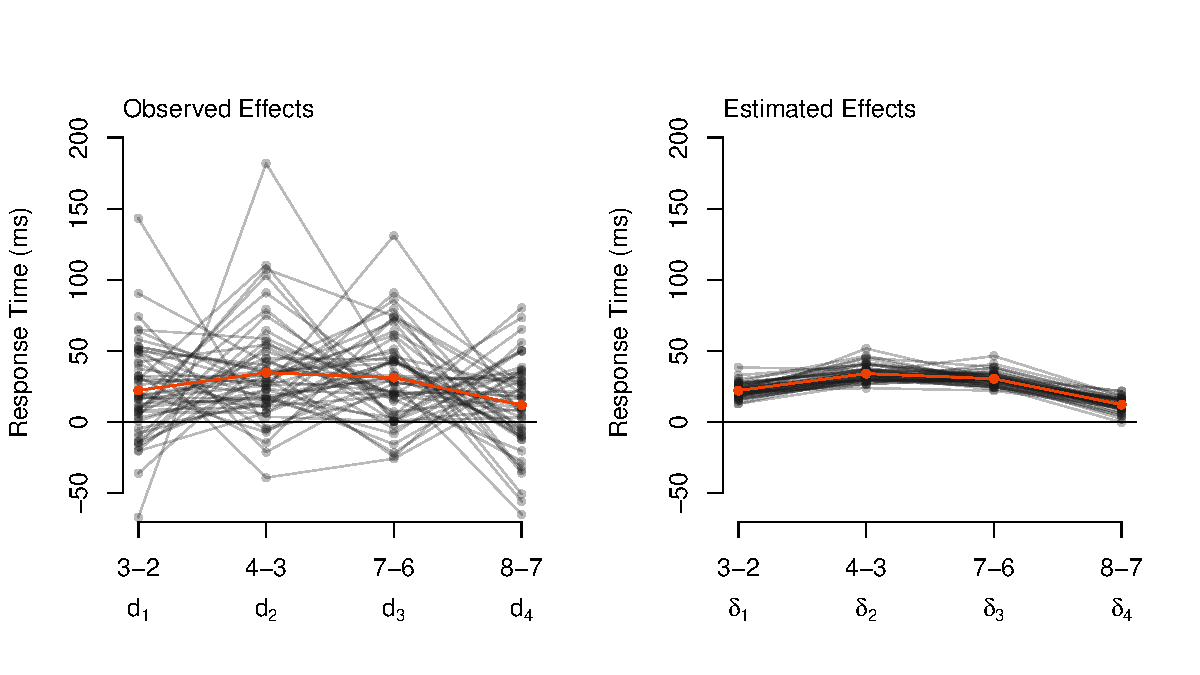
\includegraphics{t_files/figure-beamer/unnamed-chunk-7-1} \end{center}

\column{.3\textwidth}
\end{columns}

\end{frame}

\begin{frame}{Take-away for the Pragmatic Psychologist}

\vspace*{1cm}

\begin{itemize}[<+->]
\tightlist
\item
  You know a lot about ordinal predictions from theory!
\item
  Bayesian model comparison gives an accessible framework to test
  \emph{your} predictions
\item
  Bayesian analysis means you have to add value even after running your
  analysis
\item
  Are you convinced by a Bayes factor of 3-to-1?
\end{itemize}

\vspace*{1.5cm}

\begin{figure}
\hfill
\includegraphics[width = 80px]{pics/psychology.png}
\end{figure}

\end{frame}

\begin{frame}{A Step Further: Ordinal Constraint Across People}

\vspace*{1cm}

\centering \includegraphics[width = 175px]{pics/arrows.png}

\end{frame}

\begin{frame}{A step further}

\framesubtitle{Ordinal constraint across people}

\vspace*{1cm}

\begin{itemize}[<+->]
\tightlist
\item
  Stimulus strength: Does everyone truly detect bright lights faster
  than dim ones? (Most likely)
\end{itemize}

\begin{itemize}[<+->]
\tightlist
\item
  Handedness: Does everyone have a true right handed advantage? (Clearly
  no)
\end{itemize}

\begin{itemize}[<+->]
\tightlist
\item
  \textbf{Symbolic distance: Does everyone truly represent numbers as
  analog quantities? (IDK)}
\end{itemize}

\end{frame}

\begin{frame}{Does everyone?}

\vspace*{1cm}

\begin{itemize}[<+->]
\tightlist
\item
  Different Structures Yield Different Processing Interpretations
\item
  Everyone has a true positive effect \(\rightarrow\) common mechanism
  perhaps simpler explanation
\item
  Mixed effects \(\rightarrow\) strategies, perhaps complex. What
  determines who is truly positive and who is truly negative?
\end{itemize}

\vspace*{1.5cm}

\begin{figure}
\hfill
\includegraphics[width = 100px]{pics/arrows.png}
\end{figure}

\end{frame}

\begin{frame}{Symbolic Distance}

\framesubtitle{How do we represent numbers internally?}

\vspace*{.3cm}

\centering \includegraphics[width = 150px]{pics/numbers.png}

\end{frame}

\begin{frame}{How do we represent numbers internally?}

\framesubtitle{Theoretical Positions:}

\vspace*{.3cm}

\begin{enumerate}
\def\labelenumi{\arabic{enumi}.}
\tightlist
\item
  Everyones uses analog representation.
\end{enumerate}

\vspace*{.7cm}

\centering \includegraphics[width = 250px]{pics/skala.png}

\end{frame}

\begin{frame}{How do we represent numbers internally?}

\framesubtitle{Theoretical Positions:}

\vspace*{.3cm}

\begin{enumerate}
\def\labelenumi{\arabic{enumi}.}
\tightlist
\item
  Everyones uses analog representation.
\item
  Everyone uses propositional representation.
\end{enumerate}

\vspace*{.4cm}

\centering \includegraphics[width = 290px]{pics/verhaeltnis.png}

\end{frame}

\begin{frame}{How do we represent numbers internally?}

\framesubtitle{Theoretical Positions:}

\vspace*{.3cm}

\begin{enumerate}
\def\labelenumi{\arabic{enumi}.}
\tightlist
\item
  Everyones uses analog representation.
\item
  Everyone uses propositional representation.
\item
  Everyone uses priming + spreading activation.
\end{enumerate}

\vspace*{.2cm}

\centering \includegraphics[width = 250px]{pics/optinussprime.png}

\end{frame}

\begin{frame}{How do we represent numbers internally?}

\framesubtitle{Theoretical Positions:}

\vspace*{.3cm}

\begin{enumerate}
\def\labelenumi{\arabic{enumi}.}
\tightlist
\item
  Everyones uses analog representation.
\item
  Everyone uses propositional representation.
\item
  Everyone uses priming + spreading activation.
\item
  None of the above.
\end{enumerate}

\vspace*{.2cm}

\centering \includegraphics[width = 130px]{pics/whoot.png}

\end{frame}

\begin{frame}{Symbolic Distance}

\framesubtitle{Theoretical Positions as Systems of Orders}

\vspace*{.2cm}

\begin{center}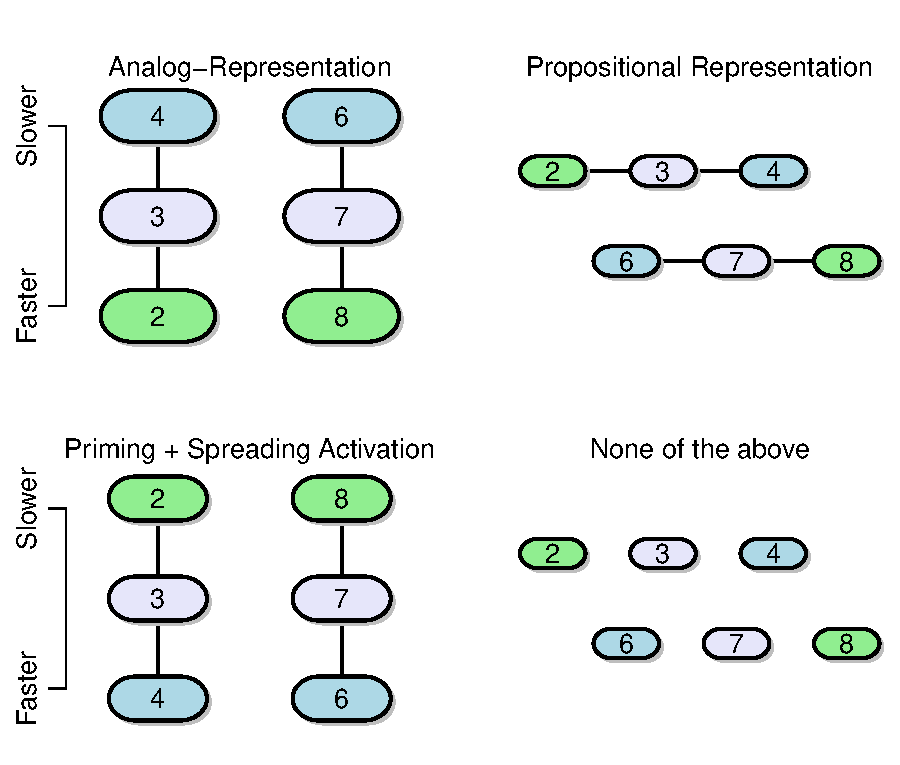
\includegraphics{t_files/figure-beamer/unnamed-chunk-8-1} \end{center}

\end{frame}

\begin{frame}{Results for ``Does Everyone'' Analysis}

\framesubtitle{Rouder, Lu, Speckman, Sun, \& Jiang (2005)}

\vspace*{.5cm}

\begin{columns}
\column{.1\textwidth}
\column{.8\textwidth}


\begin{center}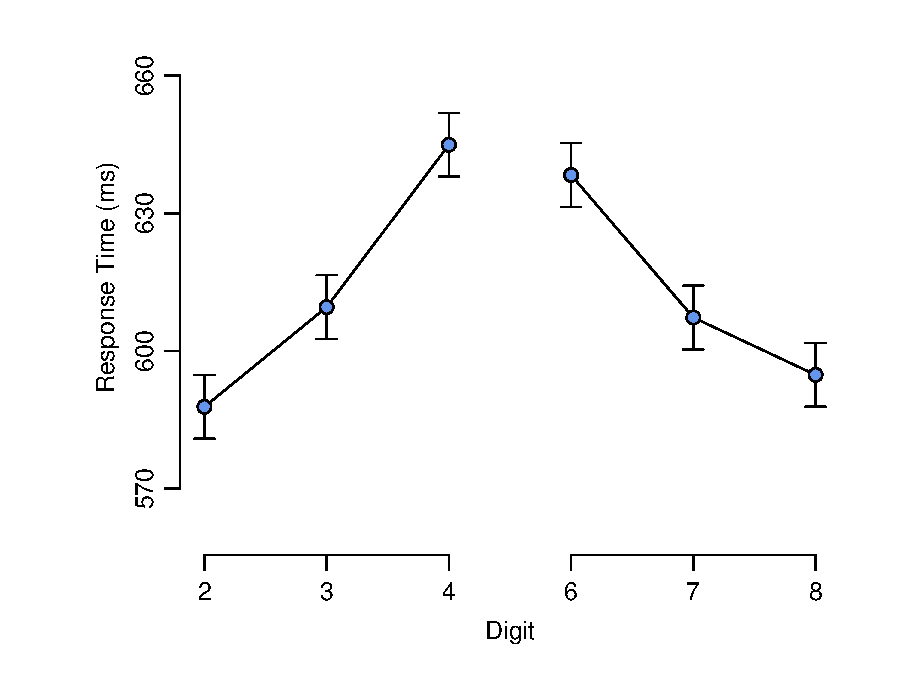
\includegraphics{t_files/figure-beamer/plot-ld5-1} \end{center}

\column{.1\textwidth}
\end{columns}

\end{frame}

\begin{frame}{Results for ``Does Everyone'' Analysis}

\framesubtitle{Rouder, Lu, Speckman, Sun, \& Jiang (2005)}

\vspace*{.5cm}

\begin{columns}
\column{.1\textwidth}
\column{.8\textwidth}


\begin{center}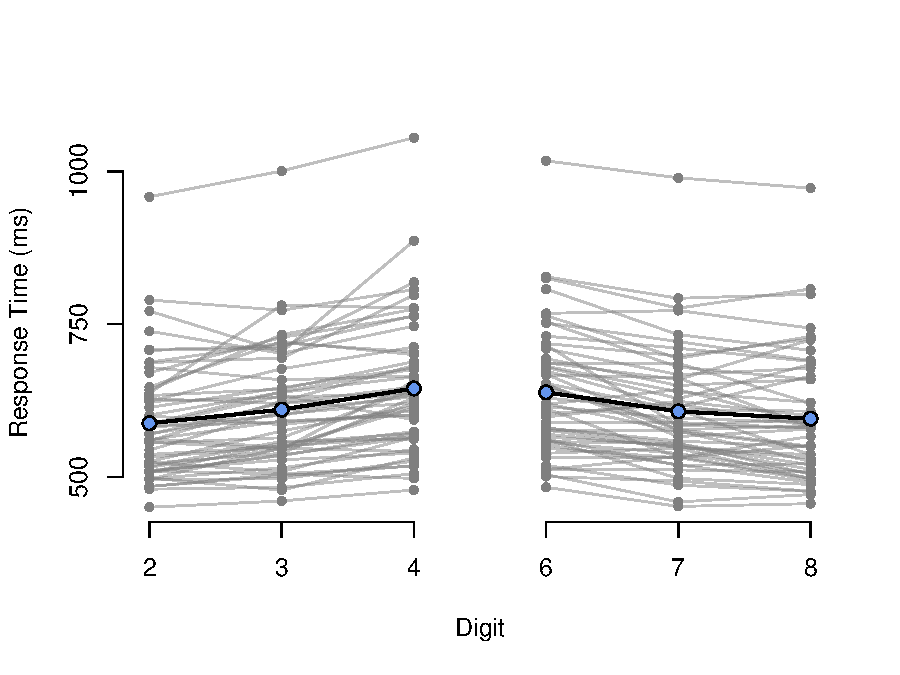
\includegraphics{t_files/figure-beamer/plot-ld5-all-1} \end{center}

\column{.1\textwidth}
\end{columns}

\end{frame}

\begin{frame}{Results for ``Does Everyone'' Analysis}

\framesubtitle{Rouder et al. (2005)}

\vspace*{1cm}

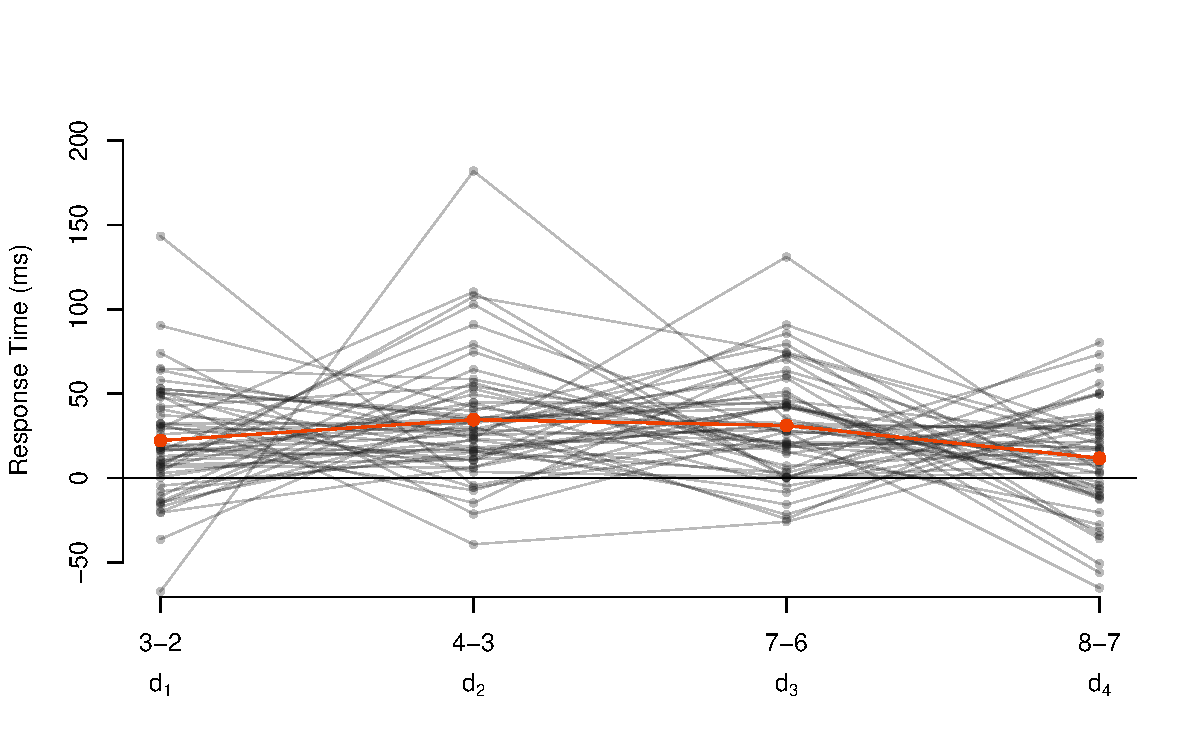
\includegraphics{t_files/figure-beamer/unnamed-chunk-9-1.pdf}

\end{frame}

\begin{frame}{Results for ``Does Everyone'' Analysis}

\vspace*{1cm}

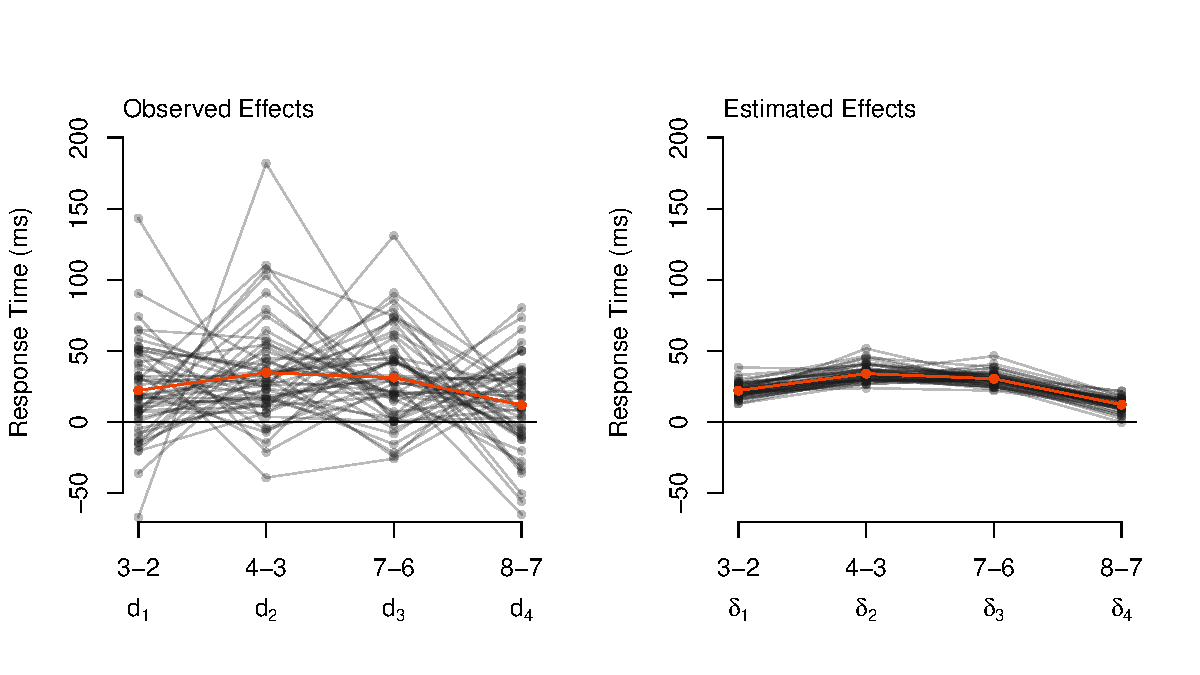
\includegraphics{t_files/figure-beamer/unnamed-chunk-10-1.pdf}

\end{frame}

\begin{frame}{Results for ``Does Everyone'' Analysis}

\vspace*{.2cm}

\begin{itemize}[<+->]
\tightlist
\item
  Preferred model: \textbf{Analog representation} model
\end{itemize}

\begin{itemize}[<+->]
\tightlist
\item
  Preferred 11.56-to-1 over the \textbf{None of the above} model
\end{itemize}

\begin{itemize}[<+->]
\tightlist
\item
  Preferred \(3 \times 10^{55}\)-to-1 over the \textbf{Propositional
  representation} model
\end{itemize}

\begin{itemize}[<+->]
\tightlist
\item
  Bayes factor for \textbf{Priming + spreading activation} model cannot
  be estimated
\end{itemize}

\centering \includegraphics[width = 200px]{pics/skala.png}

\end{frame}

\begin{frame}{Take-away for the Pragmatic Psychologist}

\vspace*{.5cm}

\begin{enumerate}[<+->]
\def\labelenumi{\arabic{enumi}.}
\tightlist
\item
  Theoretical ordinal predictions may account for everyone
\item
  ``Everyone Does'' models are parsimonious descriptions of common
  mechanisms
\item
  Bayesian analysis is the perfect tool to:
\end{enumerate}

\begin{itemize}[<+->]
\tightlist
\item
  Estimate individuals' effects with hierarchical modeling
  (visualization, diagnosis)
\item
  Assess how well each model predicts observed data using Bayes factors
\end{itemize}

\vspace*{.5cm}

\begin{figure}
\hfill
\includegraphics[width = 80px]{pics/psychology.png}
\end{figure}

\end{frame}

\begin{frame}[fragile]{Further Recources for the Pragmatic Psychologist}

\vspace*{1cm}

\begin{itemize}
\item
  Accessible book to get started with systems of orders: Hoijtink (2012)
\item
  Software packages: \texttt{bain} or \texttt{BayesFactor} for
  \texttt{R} users
\item
  ``Does everyone'' analysis: Haaf \& Rouder (2017)
\item
  Presentation and all code is available at: \color{blue}
  \href{https://tinyurl.com/OrdinalConstraint}{tinyurl.com/OrdinalConstraint}
\end{itemize}

\end{frame}

\begin{frame}{Thank You}

\vspace*{1cm}

\begin{figure}
\centering
\begin{minipage}{.5\textwidth}
  \centering
  \includegraphics[width = 110px]{pics/Fayette_Klaassen.jpg}
  
  Fayette Klaassen 
  
  (Utrecht University)
\end{minipage}%
\begin{minipage}{.5\textwidth}
  \centering
  \includegraphics[width = 170px]{pics/Jeff_Rouder.jpg}
  
  Jeff Rouder 
  
  (University of California - Irvine)
\end{minipage}
\end{figure}

\end{frame}

\section{Additional Slides}\label{additional-slides}

\begin{frame}{Preferred model}

\vspace*{1cm}

\begin{columns}
\column{.1\textwidth}
\column{.8\textwidth}


\begin{center}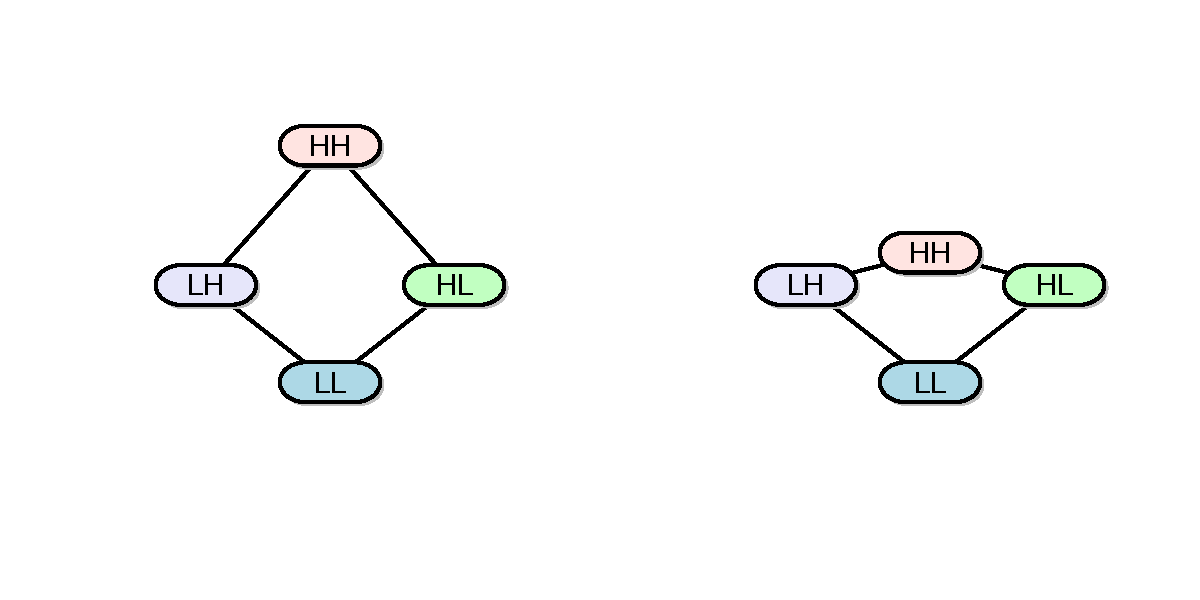
\includegraphics{t_files/figure-beamer/unnamed-chunk-11-1} \end{center}

\column{.1\textwidth}
\end{columns}

\end{frame}

\begin{frame}{References}

\scriptsize  \setlength{\parindent}{-0.5in} \setlength{\leftskip}{0.5in}

\hypertarget{refs}{}
\hypertarget{ref-Haaf:Rouder:2017}{}
Haaf, J. M., \& Rouder, J. N. (2017). Developing constraint in Bayesian
mixed models. \emph{Psychological Methods}, \emph{22}(4), 779--798.

\hypertarget{ref-Hoijtink:2012}{}
Hoijtink, H. (2012). \emph{Informative Hypotheses. Theory and Practice
for Behavioral and Social Scientists}. Boca Raton: Chapman \& Hall/CRC.

\hypertarget{ref-Rouder:etal:2005a}{}
Rouder, J. N., Lu, J., Speckman, P. L., Sun, D., \& Jiang, Y. (2005). A
hierarchical model for estimating response time distributions.
\emph{Psychonomic Bulletin and Review}, \emph{12}, 195--223.

\hypertarget{ref-Rouder:etal:2012}{}
Rouder, J. N., Morey, R. D., Speckman, P. L., \& Province, J. M. (2012).
Default Bayes factors for ANOVA designs. \emph{Journal of Mathematical
Psychology}, \emph{56}, 356--374. Retrieved from
\url{http://dx.doi.org/10.1016/j.jmp.2012.08.001}

\hypertarget{ref-Ryan:etal:2013}{}
Ryan, R. S., Wilde, M., \& Crist, S. (2013). Compared to a small,
supervised lab experiment, a large, unsupervised web-based experiment on
a previously unknown effect has benefits that outweigh its potential
costs. \emph{Computers in Human Behavior}, \emph{29}(4), 1295--1301.

\end{frame}

\end{document}
